\documentclass[11pt, aspectratio=169]{beamer}

% LuaLaTeXで日本語を使うための必須パッケージ
\usepackage{luatexja}

% 便利な追加パッケージ
\usepackage{tikz}
\usetikzlibrary{shapes.symbols}
\usetikzlibrary{positioning, calc, shapes.geometric} % shapes.geometric を追加
\usepackage{booktabs}   % 表の罫線
\usepackage{tikz}       % 図形描画
\usepackage{listings}   % ソースコード挿入
\lstset{
  basicstyle=\ttfamily\scriptsize,
  frame=single,
  breaklines=true,
  numbers=left,
  numberstyle=\tiny
}

% テーマとカラーテーマの設定
\usetheme{Madrid}
\usecolortheme{orchid}

% セクション開始時の自動表紙（扉絵）設定
\AtBeginSection[]{
  \begin{frame}
    \vfill
    \centering
    \begin{beamercolorbox}[sep=8pt,center,shadow=true,rounded=true]{title}
      \usebeamerfont{title}\insertsectionhead\par%
    \end{beamercolorbox}
    \vfill
  \end{frame}
}

% タイトル情報
\title{研究室セミナー第2回}
\subtitle{SAGIN}
\author{学籍番号(Student ID): 1280391 \\ 氏名(Name): 細川夏風(Hosokawa Natsuka)}
\institute{高知工科大学(Kochi Univ of Tech)}
\date{\today}

\begin{document}

% タイトルスライド
\begin{frame}
    \titlepage
\end{frame}

% 目次スライド
\begin{frame}{目次}
    \tableofcontents
\end{frame}

% ==========================================
% ここから本文
% ==========================================

\section{はじめに / Intro}

\subsection{SAGINについて / About SAGIN}

\begin{frame}{SAGINについて}
  \begin{columns}[c]
    \begin{column}{0.4\textwidth}
      \texttt{SAGIN}とは，宇宙・航空・地上統合ネットワークのことである．衛星システム，航空ネットワーク，地上通信を統合する新しいネットワークアーキテクチャである．

      これにより以下の\texttt{6G}要件を満たすことが期待されている．
      \begin{itemize}
        \item 広域アクセス
        \item 大規模接続
        \item 高精度測位
      \end{itemize}
    \end{column}
    \begin{column}{0.6\textwidth}
      \begin{center}
        % resizeboxで図の横幅をカラムの幅(\linewidth)に合わせる
        \resizebox{\linewidth}{!}{
          \begin{tikzpicture}[
            node distance=2.5cm,
            segment/.style={draw, rounded corners, align=center, minimum width=8cm, minimum height=1.2cm, font=\sffamily\bfseries},
            link/.style={<->, thick, >=stealth}
        ]
            % ノードの定義
            \node[segment, fill=blue!15] (space) {宇宙ネットワーク (Space Network)};
            \node[segment, fill=green!15, below of=space] (air) {航空ネットワーク (Air Network)};
            \node[segment, fill=orange!15, below of=air] (ground) {地上ネットワーク (Ground Network)};

            % 垂直方向のリンク
            \draw[link] (space.south) -- (air.north) node[midway, right] {\small Space-Air};
            \draw[link] (air.south) -- (ground.north) node[midway, right] {\small Air-Ground};

            % 宇宙と地上の直接リンク
            \draw[link] (space.west) to[out=210, in=150] node[midway, left] {\small Space-Ground} (ground.west);
          \end{tikzpicture}
        }
      \end{center}
    \end{column}
  \end{columns}
\end{frame}

\begin{frame}{About SAGIN}
  \begin{columns}[c]
    \begin{column}{0.4\textwidth}
      \texttt{SAGIN} stands for Space-Air-Ground Integrated Network. It is a novel network architecture that integrates satellite systems, air networks, and terrestrial communications.

      It is expected to meet various \texttt{6G} requirements, including:
      \begin{itemize}
        \item Wide-area broadband access
        \item Large-scale connectivity
        \item High-precision positioning
      \end{itemize}
    \end{column}
    \begin{column}{0.6\textwidth}
      \begin{center}
        % Use resizebox to scale the TikZ diagram to column width
        \resizebox{\linewidth}{!}{
          \begin{tikzpicture}[
            node distance=2.5cm,
            segment/.style={draw, rounded corners, align=center, minimum width=8cm, minimum height=1.2cm, font=\sffamily\bfseries},
            link/.style={<->, thick, >=stealth}
        ]
            % Definition of nodes
            \node[segment, fill=blue!15] (space) {Space Network};
            \node[segment, fill=green!15, below of=space] (air) {Air Network};
            \node[segment, fill=orange!15, below of=air] {Ground Network};

            % Vertical links
            \draw[link] (space.south) -- (air.north) node[midway, right] {\small Space-Air};
            \draw[link] (air.south) -- (ground.north) node[midway, right] {\small Air-Ground};

            % Direct link between Space and Ground
            \draw[link] (space.west) to[out=210, in=150] node[midway, left] {\small Space-Ground} (ground.west);
          \end{tikzpicture}
        }
      \end{center}
    \end{column}
  \end{columns}
\end{frame}

\subsection{なぜSAGINが必要なのか / Why we need SAGIN}

\begin{frame}{なぜSAGINが必要なのか / Why we need SAGIN}
  より広域により低遅延で通信を実現しようとした場合，現行の通信方式ではアクセスの柔軟性も低いうえに遅延が大きいという課題がある．

  そのため，\texttt{SAGIN}を導入し，シームレスに様々な領域を超えた統合ネットワークを構築する必要がある．

  \vspace{1cm}

  When aiming for communication with wider coverage and lower latency, current communication systems face the challenges of poor access flexibility and high latency.

  Therefore, it is necessary to introduce \texttt{SAGIN} and build an integrated network that seamlessly transcends various domains.
\end{frame}

\section{アーキテクチャ / Architecture}

\begin{frame}{宇宙ネットワーク}
  \begin{columns}[c]
    \begin{column}{0.5\textwidth}
      このネットワークは異なる軌道にある衛星と地上の基地局，ネットワークオペレータ，制御センターなどの対応する地上のインフラ施設や設備で構成されている．衛星は高度に応じて，静止衛星(\texttt{GEO})，中軌道衛星(\texttt{MEO})，低軌道衛星(\texttt{LEO})の$3$つのカテゴリに分類されている．

      \vspace{1em}

      これらの衛星同士が多層衛星ネットワーク(\texttt{MLSN})を構成している．これには衛星間リンク(\texttt{ISL})や層間リンク(\texttt{ILL})などの複数リンクタイプが存在する．
    \end{column}
    \begin{column}{0.5\textwidth}
      \begin{center}
        % 0.65 * 1.07 = 約0 に拡大
        \resizebox{!}{0.75\textheight}{
        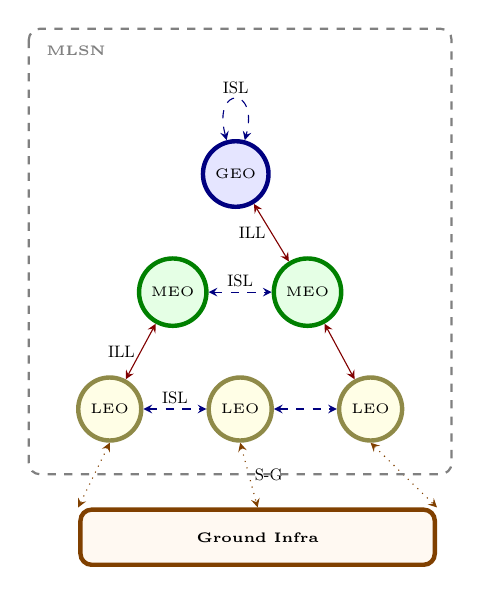
\begin{tikzpicture}[
            node distance=0.5cm and 0.8cm,
            sat/.style={circle, draw, minimum size=0.6cm, align=center, font=\tiny, ultra thick},
            geo/.style={sat, fill=blue!10, draw=blue!50!black},
            meo/.style={sat, fill=green!10, draw=green!50!black},
            leo/.style={sat, fill=yellow!10, draw=yellow!50!black},
            ground/.style={rectangle, draw, rounded corners, fill=orange!5, minimum width=4.5cm, minimum height=0.7cm, align=center, font=\tiny\bfseries, ultra thick, draw=orange!50!black},
            link/.style={<->, thin, >=stealth},
            isl/.style={link, blue!50!black, dashed},
            ill/.style={link, red!50!black},
            glink/.style={link, orange!50!black, dotted}
        ]
            % --- ノード配置 ---
            \node[ground] (infra) {Ground Infra};
            \node[leo, above=1.2cm of infra.west, xshift=0.4cm] (leo1) {LEO};
            \node[leo, right=of leo1] (leo2) {LEO};
            \node[leo, right=of leo2] (leo3) {LEO};
            \node[meo, above=0.6cm of leo1, xshift=0.8cm] (meo1) {MEO};
            \node[meo, right=of meo1] (meo2) {MEO};
            \node[geo, above=0.6cm of meo1, xshift=0.8cm] (geo1) {GEO};

            % --- リンク描画 ---
            \draw[isl] (geo1) to[loop above] node[above, black, scale=0.6] {ISL} (geo1); 
            \draw[isl] (meo1) -- node[above, black, scale=0.6] {ISL} (meo2);
            \draw[isl] (leo1) -- node[above, black, scale=0.6] {ISL} (leo2);
            \draw[isl] (leo2) -- (leo3);
            
            \draw[ill] (geo1) -- node[midway, left, black, scale=0.6] {ILL} (meo2);
            \draw[ill] (meo1) -- node[midway, left, black, scale=0.6] {ILL} (leo1);
            \draw[ill] (meo2) -- (leo3);
            
            \draw[glink] (leo1.south) -- (infra.north west);
            \draw[glink] (leo2.south) -- node[midway, right, black, scale=0.6] {S-G} (infra.north);
            \draw[glink] (leo3.south) -- (infra.north east);

            % --- MLSN枠の修正（バランス調整） ---
            % 左端をleo1、右端をleo3、上端をgeo1(のISL分)を基準にして左右対称に
            \draw[dashed, gray, thick, rounded corners] 
              ($(leo1.west |- geo1.north)+(-0.6cm,1.4cm)$) rectangle ($(leo3.east |- leo3.south)+(0.6cm,-0.4cm)$);
            
            \node[anchor=north west, font=\tiny\bfseries, gray] 
              at ($(leo1.west |- geo1.north)+(-0.5cm,1.3cm)$) {MLSN};

        \end{tikzpicture}
        }
      \end{center}
    \end{column}
  \end{columns}
\end{frame}

\subsection{宇宙ネットワーク / Space Network}

\begin{frame}{Space Network}
  \begin{columns}[c]
    \begin{column}{0.5\textwidth}
      \small % 英語は文字数が多くなりやすいため、少しだけ小さくすると収まりが良いです
      This network consists of satellites in various orbits and corresponding ground infrastructure facilities and equipment, such as base stations, network operators, and control centers.

      \vspace{1em}
      Satellites are classified into three categories based on altitude: Geostationary Earth Orbit (\texttt{GEO}), Medium Earth Orbit (\texttt{MEO}), and Low Earth Orbit (\texttt{LEO}).

      \vspace{1em}
      These satellites form a Multi-Layer Satellite Network (\texttt{MLSN}), which utilizes multiple link types such as Inter-Satellite Links (\texttt{ISL}) and Inter-Layer Links (\texttt{ILL}).
    \end{column}
    \begin{column}{0.5\textwidth}
      \begin{center}
        \resizebox{!}{0.75\textheight}{
        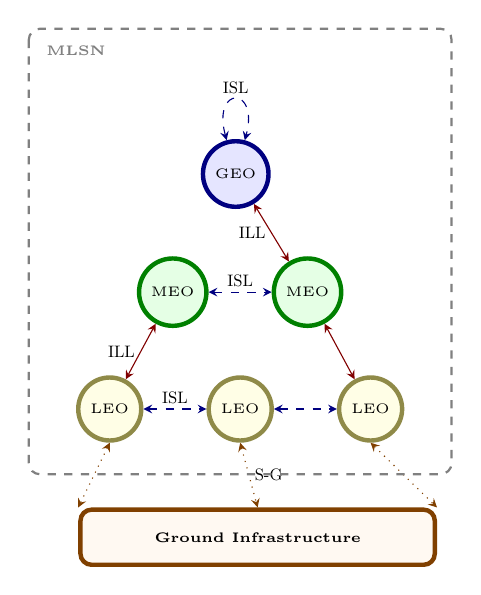
\begin{tikzpicture}[
            node distance=0.5cm and 0.8cm,
            sat/.style={circle, draw, minimum size=0.6cm, align=center, font=\tiny, ultra thick},
            geo/.style={sat, fill=blue!10, draw=blue!50!black},
            meo/.style={sat, fill=green!10, draw=green!50!black},
            leo/.style={sat, fill=yellow!10, draw=yellow!50!black},
            ground/.style={rectangle, draw, rounded corners, fill=orange!5, minimum width=4.5cm, minimum height=0.7cm, align=center, font=\tiny\bfseries, ultra thick, draw=orange!50!black},
            link/.style={<->, thin, >=stealth},
            isl/.style={link, blue!50!black, dashed},
            ill/.style={link, red!50!black},
            glink/.style={link, orange!50!black, dotted}
        ]
            % --- Node Placement ---
            \node[ground] (infra) {Ground Infrastructure};
            \node[leo, above=1.2cm of infra.west, xshift=0.4cm] (leo1) {LEO};
            \node[leo, right=of leo1] (leo2) {LEO};
            \node[leo, right=of leo2] (leo3) {LEO};
            \node[meo, above=0.6cm of leo1, xshift=0.8cm] (meo1) {MEO};
            \node[meo, right=of meo1] (meo2) {MEO};
            \node[geo, above=0.6cm of meo1, xshift=0.8cm] (geo1) {GEO};

            % --- Link Drawing ---
            \draw[isl] (geo1) to[loop above] node[above, black, scale=0.6] {ISL} (geo1);
            \draw[isl] (meo1) -- node[above, black, scale=0.6] {ISL} (meo2);
            \draw[isl] (leo1) -- node[above, black, scale=0.6] {ISL} (leo2);
            \draw[isl] (leo2) -- (leo3);

            \draw[ill] (geo1) -- node[midway, left, black, scale=0.6] {ILL} (meo2);
            \draw[ill] (meo1) -- node[midway, left, black, scale=0.6] {ILL} (leo1);
            \draw[ill] (meo2) -- (leo3);

            \draw[glink] (leo1.south) -- (infra.north west);
            \draw[glink] (leo2.south) -- node[midway, right, black, scale=0.6] {S-G} (infra.north);
            \draw[glink] (leo3.south) -- (infra.north east);

            % --- MLSN Box Correction ---
            \draw[dashed, gray, thick, rounded corners]
              ($(leo1.west |- geo1.north)+(-0.6cm,1.4cm)$) rectangle ($(leo3.east |- leo3.south)+(0.6cm,-0.4cm)$);

            \node[anchor=north west, font=\tiny\bfseries, gray]
              at ($(leo1.west |- geo1.north)+(-0.5cm,1.3cm)$) {MLSN};

        \end{tikzpicture}
        }
      \end{center}
    \end{column}
  \end{columns}
\end{frame}

\begin{frame}[c]{静止衛星 (GEO) / Geostationary Earth Orbit}
  \begin{columns}[c]
    \begin{column}{0.45\textwidth}
      地上に対して固定された高軌道の位置に存在する．単一の衛星で地球の面積の 42\% をカバー可能．3 ～ 4 機で極地を含みカバー可能．ただ，一方向の遅延が大きく約 270ms 程となっている．

      \vspace{1em}
      \textit{GEO satellites are located in a fixed high-altitude orbit relative to the ground. A single satellite can cover 42\% of the Earth's area, and 3--4 satellites can provide coverage including the polar regions. However, the one-way delay is large, at approximately 270ms.}
    \end{column}

    \begin{column}{0.5\textwidth}
      \begin{center}
        \resizebox{!}{0.65\textheight}{
        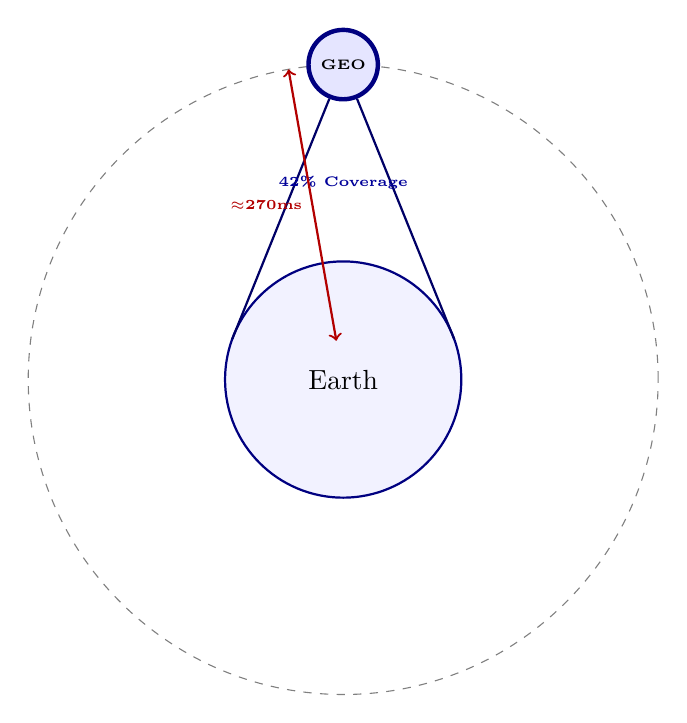
\begin{tikzpicture}[sat/.style={circle, fill=blue!10, draw=blue!50!black, ultra thick, minimum size=0.8cm, font=\tiny\bfseries}]
            \draw[fill=blue!5, draw=blue!50!black, thick] (0,0) circle (1.5);
            \node at (0,0) {Earth};
            \draw[dashed, gray] (0,0) circle (4);
            \node[sat] (s) at (90:4) {GEO};
            \draw[blue!40!black, thick] (s) -- (160:1.5);
            \draw[blue!40!black, thick] (s) -- (20:1.5);
            \node[blue!60!black, font=\tiny\bfseries] at (90:2.5) {42\% Coverage};
            \draw[<->, red!70!black, thick] (100:0.5) -- (100:4) node[midway, left, font=\tiny\bfseries] {$\approx$270ms};
        \end{tikzpicture}
        }
      \end{center}
    \end{column}
  \end{columns}
\end{frame}

\begin{frame}[c]{中軌道衛星 (MEO) / Medium Earth Orbit}
  \begin{columns}[c]
    \begin{column}{0.5\textwidth}
      \small
      高度が 2000km ～ 20000km の位置し，地球面積の 12\% ～ 38\% 程をカバーし，10 機以上で全体をカバー可能．高帯域幅，低コスト低遅延を実現可能に設定されている．システムの容量が最大 15Gbps になる．文献 \cite{chen2023space} では，遅延は 110ms とされている．

      \vspace{1em}
      \textit{Located at altitudes of 2,000km to 20,000km, MEO satellites cover about 12\% to 38\% of the Earth's area and can cover the entire globe with 10 or more satellites. They are designed to achieve high bandwidth, low cost, and low latency. The system capacity reaches up to 15Gbps. In literature \cite{chen2023space}, the latency is stated as 110ms.}
    \end{column}

    \begin{column}{0.5\textwidth}
      \begin{center}
        \resizebox{!}{0.65\textheight}{
        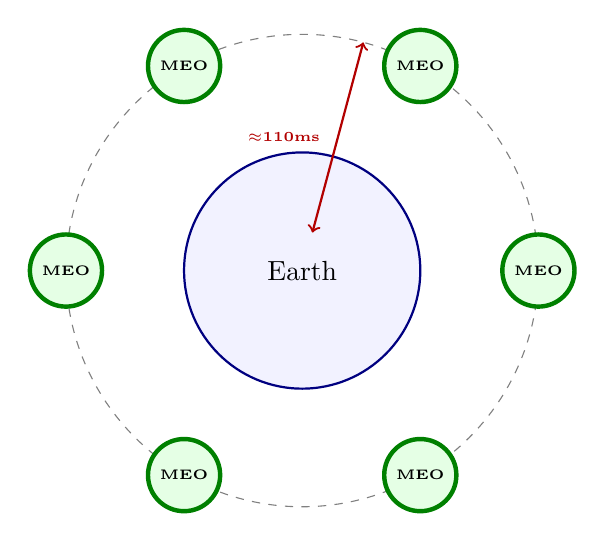
\begin{tikzpicture}[sat/.style={circle, fill=green!10, draw=green!50!black, ultra thick, minimum size=0.6cm, font=\tiny\bfseries}]
            \draw[fill=blue!5, draw=blue!50!black, thick] (0,0) circle (1.5);
            \node at (0,0) {Earth};
            \draw[dashed, gray] (0,0) circle (3);
            \foreach \a in {0, 60, 120, 180, 240, 300} {
                \node[sat] at (\a:3) {MEO};
            }
            \draw[<->, red!70!black, thick] (75:0.5) -- (75:3) node[midway, left, font=\tiny\bfseries, xshift=-0.1cm] {$\approx$110ms};
        \end{tikzpicture}
        }
      \end{center}
    \end{column}
  \end{columns}
\end{frame}

\begin{frame}[c]{低軌道衛星 (LEO) / Low Earth Orbit}
  \begin{columns}[c]
    \begin{column}{0.45\textwidth}
      低コストで構築可能だが，グローバル通信を実現するためには多数の衛星が必要．伝播距離が短いため，遅延が 40ms 未満と小さい．地上に対して移動速度が大きいため，通信を安定させることが難しい．

      \vspace{1em}
      \textit{LEO satellites can be built at low cost but require a large number of satellites to achieve global communication. Due to the short propagation distance, the delay is small, less than 40ms. Since the movement speed relative to the ground is high, it is difficult to stabilize communication.}
    \end{column}

    \begin{column}{0.5\textwidth}
      \begin{center}
        \resizebox{!}{0.65\textheight}{
        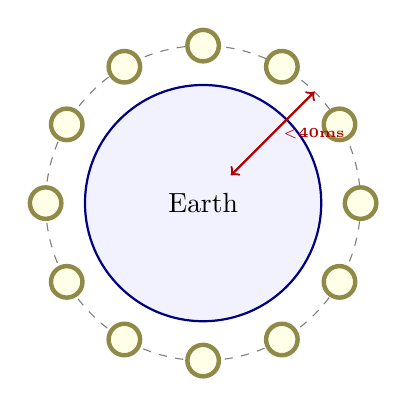
\begin{tikzpicture}[sat/.style={circle, fill=yellow!10, draw=yellow!50!black, ultra thick, minimum size=0.4cm, font=\tiny\bfseries}]
            \draw[fill=blue!5, draw=blue!50!black, thick] (0,0) circle (1.5);
            \node at (0,0) {Earth};
            \draw[dashed, gray] (0,0) circle (2);
            \foreach \a in {0, 30, 60, 90, 120, 150, 180, 210, 240, 270, 300, 330} {
                \node[sat] at (\a:2) {};
            }
            \draw[<->, red!70!black, thick] (45:0.5) -- (45:2) node[midway, right, font=\tiny\bfseries] {$<$40ms};
        \end{tikzpicture}
        }
      \end{center}
    \end{column}
  \end{columns}
\end{frame}

\subsection{航空ネットワーク / Air Network}

\begin{frame}[c]{航空ネットワーク}
  \begin{columns}[c]
    \begin{column}{0.5\textwidth}
      このネットワークは航空機器（航空機，気球，\texttt{UAV}：無人航空機）をキャリアとして使用し，情報の送信、処理を行うモバイルシステムである．
      
      \vspace{0.5em}
      宇宙ネットワークと同様に高度によって，高高度プラットフォーム (\texttt{HAPs})，低高度プラットフォーム (\texttt{LAPs}) に分類できる．
      
      \vspace{0.5em}
      地上基地局と比較して展開が容易でカバー範囲が広く，地域のワイヤレスアクセスを提供可能である．また，構築コストは宇宙ネットワークの運用よりも遥かに低く抑えられる．
    \end{column}

    \begin{column}{0.48\textwidth}
      \begin{center}
        \resizebox{!}{0.65\textheight}{
        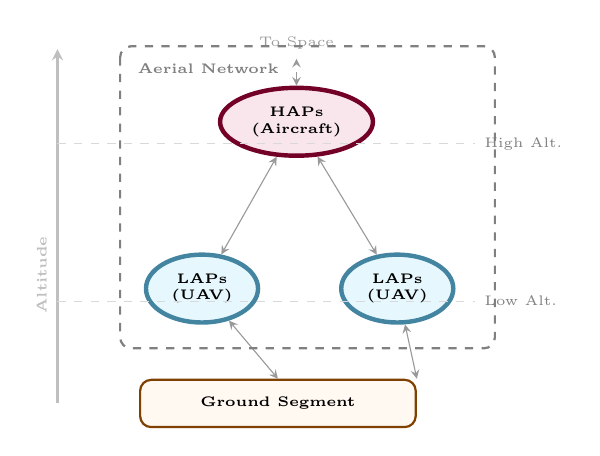
\begin{tikzpicture}[
            node distance=0.6cm and 1.0cm,
            ground/.style={rectangle, draw, rounded corners, fill=orange!5, minimum width=3.5cm, minimum height=0.6cm, align=center, font=\tiny\bfseries, thick, draw=orange!50!black},
            platform/.style={ellipse, draw, ultra thick, minimum width=1.2cm, minimum height=0.7cm, align=center, font=\tiny\bfseries},
            haps/.style={platform, fill=purple!10, draw=purple!60!black},
            laps/.style={platform, fill=cyan!10, draw=cyan!60!black},
            link/.style={<->, thin, >=stealth, gray!80},
            axis/.style={->, thick, >=stealth, gray!50}
        ]
            % --- 1. ノード配置（xshiftを増やして軸から離す） ---
            \node[ground] (infra) at (1,0) {Ground Segment};
            
            \node[laps, above=1.0cm of infra.west, xshift=0.8cm] (lap1) {LAPs\\(UAV)};
            \node[laps, right=of lap1] (lap2) {LAPs\\(UAV)};
            
            \node[haps, above=1.2cm of lap1, xshift=1.2cm] (hap1) {HAPs\\(Aircraft)};

            % --- 2. リンク ---
            \draw[link] (hap1) -- (lap1);
            \draw[link] (hap1) -- (lap2);
            \draw[link] (lap1) -- (infra.north);
            \draw[link] (lap2) -- (infra.north east);
            \draw[link, dashed] (hap1) -- ++(0,0.8) node[above, font=\tiny] {To Space};

            % --- 3. 高度軸（位置を左にオフセット） ---
            \draw[axis] (-1.8,0) -- (-1.8,4.5) node[midway, left, rotate=90, font=\tiny\bfseries, yshift=0.2cm] {Altitude};
            \draw[dashed, gray!30] (-1.8,1.3) -- (3.5,1.3) node[right, font=\tiny, gray] {Low Alt.};
            \draw[dashed, gray!30] (-1.8,3.3) -- (3.5,3.3) node[right, font=\tiny, gray] {High Alt.};

            % --- 4. 範囲（枠も重ならないように調整） ---
            \draw[dashed, gray, thick, rounded corners] 
              ($(lap1.west |- hap1.north)+(-0.3cm,0.5cm)$) rectangle ($(lap2.east |- lap1.south)+(0.5cm,-0.3cm)$);
            \node[anchor=north west, font=\tiny\bfseries, gray] 
              at ($(lap1.west |- hap1.north)+(-0.2cm,0.4cm)$) {Aerial Network};

        \end{tikzpicture}
        }
      \end{center}
    \end{column}
  \end{columns}
\end{frame}

\begin{frame}[c]{Aerial Network}
  \begin{columns}[c]
    \begin{column}{0.5\textwidth}
      This network is a mobile system that uses aerial equipment (aircraft, balloons, and, \texttt{UAVs}: Unmanned Aerial Vehicles) as carriers to transmit and process information.

      \vspace{0.5em}
      Similar to space networks, it can be classified into High Altitude Platforms (\texttt{HAPs}) and Low Altitude Platforms (\texttt{LAPs}) based on altitude.

      \vspace{0.5em}
      Compared to ground network base stations, aerial networks are easier to deploy and offer wider coverage. They can provide regional wireless access. At the same time, the deployment cost is significantly lower than that of operating a space network.
    \end{column}

    \begin{column}{0.48\textwidth}
      \begin{center}
        \resizebox{!}{0.65\textheight}{
        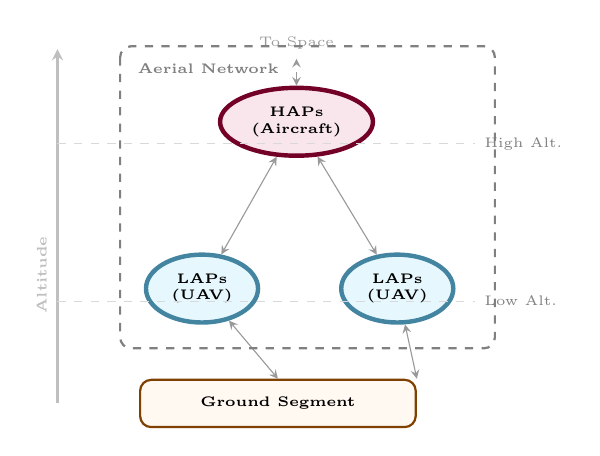
\begin{tikzpicture}[
            node distance=0.6cm and 1.0cm,
            ground/.style={rectangle, draw, rounded corners, fill=orange!5, minimum width=3.5cm, minimum height=0.6cm, align=center, font=\tiny\bfseries, thick, draw=orange!50!black},
            platform/.style={ellipse, draw, ultra thick, minimum width=1.2cm, minimum height=0.7cm, align=center, font=\tiny\bfseries},
            haps/.style={platform, fill=purple!10, draw=purple!60!black},
            laps/.style={platform, fill=cyan!10, draw=cyan!60!black},
            link/.style={<->, thin, >=stealth, gray!80},
            axis/.style={->, thick, >=stealth, gray!50}
        ]
            % --- Node Placement ---
            \node[ground] (infra) at (1,0) {Ground Segment};
            \node[laps, above=1.0cm of infra.west, xshift=0.8cm] (lap1) {LAPs\\(UAV)};
            \node[laps, right=of lap1] (lap2) {LAPs\\(UAV)};
            \node[haps, above=1.2cm of lap1, xshift=1.2cm] (hap1) {HAPs\\(Aircraft)};

            % --- Links ---
            \draw[link] (hap1) -- (lap1);
            \draw[link] (hap1) -- (lap2);
            \draw[link] (lap1) -- (infra.north);
            \draw[link] (lap2) -- (infra.north east);
            \draw[link, dashed] (hap1) -- ++(0,0.8) node[above, font=\tiny] {To Space};

            % --- Altitude Axis (Offset to the left) ---
            \draw[axis] (-1.8,0) -- (-1.8,4.5) node[midway, left, rotate=90, font=\tiny\bfseries, yshift=0.2cm] {Altitude};
            \draw[dashed, gray!30] (-1.8,1.3) -- (3.5,1.3) node[right, font=\tiny, gray] {Low Alt.};
            \draw[dashed, gray!30] (-1.8,3.3) -- (3.5,3.3) node[right, font=\tiny, gray] {High Alt.};

            % --- Box ---
            \draw[dashed, gray, thick, rounded corners]
              ($(lap1.west |- hap1.north)+(-0.3cm,0.5cm)$) rectangle ($(lap2.east |- lap1.south)+(0.5cm,-0.3cm)$);
            \node[anchor=north west, font=\tiny\bfseries, gray]
              at ($(lap1.west |- hap1.north)+(-0.2cm,0.4cm)$) {Aerial Network};

        \end{tikzpicture}
        }
      \end{center}
    \end{column}
  \end{columns}
\end{frame}

\begin{frame}[c]{高高度・低高度プラットフォーム}
  \begin{columns}[c]
    \begin{column}{0.5\textwidth}
      \small
      \begin{itemize}
        \item \texttt{HAPs} の役割

        衛星との接続にも用いられ，分散型のデータセンターとして機能している．経路の記録やお互いの監視などを行う．これらの情報は衛星と通信を行うために重要である．地上とのワイヤレスでの接続のためのサービスを提供するためにも用いられる．
      \item \texttt{LAPs} の役割

        このプラットフォーム\texttt{UAV}は重要な役割を持っており，\texttt{HAPs}より柔軟性が高い．適切な通信管理を行うことによって通信のオーバヘッドを減少させることができる．\texttt{UAV}は様々な通信の分散処理能力の向上や移動体の基地局としてモバイルのクライドコンピューティングのシステムとしてももいいることができると考えられている．
      \end{itemize}
    \end{column}

    \begin{column}{0.48\textwidth}
      \begin{center}
        \resizebox{!}{0.6\textheight}{
        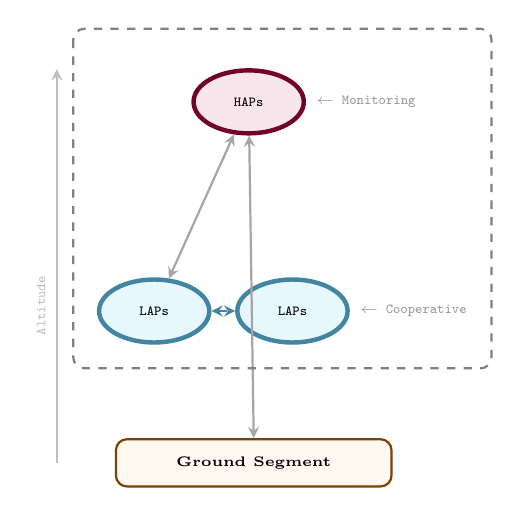
\begin{tikzpicture}[
            node distance=0.8cm and 1.2cm,
            platform/.style={ellipse, draw, ultra thick, minimum width=1.4cm, minimum height=0.8cm, align=center, font=\tiny\ttfamily},
            haps/.style={platform, fill=purple!10, draw=purple!60!black},
            laps/.style={platform, fill=cyan!10, draw=cyan!60!black},
            infra/.style={rectangle, draw, rounded corners, fill=orange!5, minimum width=3.5cm, minimum height=0.6cm, align=center, font=\tiny\bfseries, thick, draw=orange!50!black},
            label/.style={font=\tiny\ttfamily, gray!80},
            link/.style={<->, thick, >=stealth, gray!70},
            axis/.style={->, thick, >=stealth, gray!50}
        ]
            % --- ノード配置 ---
            \node[infra] (ground) at (1.5,0) {Ground Segment};
            \node[laps, above=1.5cm of ground.west, xshift=0.5cm] (lap1) {LAPs};
            \node[laps, right=0.3cm of lap1] (lap2) {LAPs};
            \draw[link, dashed, cyan!60!black] (lap1) -- (lap2);
            \node[haps, above=1.8cm of lap1, xshift=1.2cm] (hap1) {HAPs};

            % --- リンクとラベル ---
            \draw[link] (hap1) -- (lap1);
            \draw[link] (hap1) -- (ground.north);
            \draw[axis] (-1.0,0) -- (-1.0,5.0) node[midway, left, rotate=90, font=\tiny\ttfamily, yshift=0.2cm] {Altitude};
            \node[label, anchor=west] at (hap1.east) {$\leftarrow$ Monitoring};
            \node[label, anchor=west] at (lap2.east) {$\leftarrow$ Cooperative};

            % 範囲枠
            \draw[dashed, gray, thick, rounded corners]
              ($(lap1.west |- hap1.north)+(-0.3cm,0.5cm)$) rectangle ($(lap2.east |- lap1.south)+(1.8cm,-0.3cm)$);
        \end{tikzpicture}
        }
      \end{center}
    \end{column}
  \end{columns}
\end{frame}

\begin{frame}[c]{High and Low Altitude Platforms}
  \begin{columns}[c]
    \begin{column}{0.5\textwidth}
      \scriptsize
      \begin{itemize}
        \item Roles of \texttt{HAPs} \\
        They are used for connections with satellites and function as distributed data centers. They perform tasks such as recording trajectories and mutual monitoring. This information is important for conducting communication with satellites. They are also used to provide services for wireless connections with the ground.

        \vspace{0.5em}
        \item Roles of \texttt{LAPs} \\
        \texttt{UAV}s are mainly used for this platform, offering higher flexibility than \texttt{HAPs}. Communication overhead can be reduced by performing appropriate communication management. \texttt{UAV}s play an important role in this platform; it is considered that they can be used to improve various distributed processing capabilities of communications and serve as mobile base stations for mobile cloud computing systems.
      \end{itemize}
    \end{column}

    \begin{column}{0.48\textwidth}
      \begin{center}
        \resizebox{!}{0.6\textheight}{
        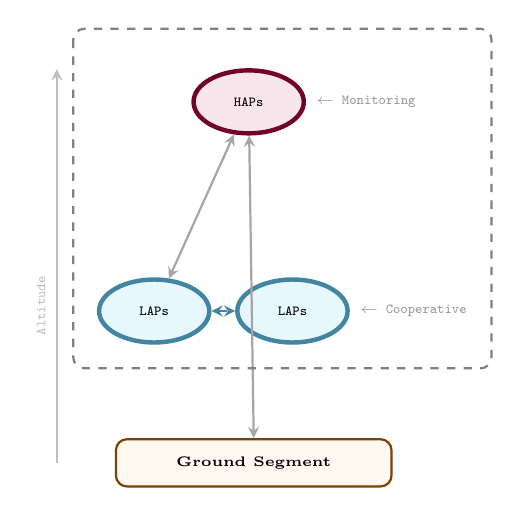
\begin{tikzpicture}[
            node distance=0.8cm and 1.2cm,
            platform/.style={ellipse, draw, ultra thick, minimum width=1.4cm, minimum height=0.8cm, align=center, font=\tiny\ttfamily},
            haps/.style={platform, fill=purple!10, draw=purple!60!black},
            laps/.style={platform, fill=cyan!10, draw=cyan!60!black},
            infra/.style={rectangle, draw, rounded corners, fill=orange!5, minimum width=3.5cm, minimum height=0.6cm, align=center, font=\tiny\bfseries, thick, draw=orange!50!black},
            label/.style={font=\tiny\ttfamily, gray!80},
            link/.style={<->, thick, >=stealth, gray!70},
            axis/.style={->, thick, >=stealth, gray!50}
        ]
            % --- Node Placement ---
            \node[infra] (ground) at (1.5,0) {Ground Segment};
            \node[laps, above=1.5cm of ground.west, xshift=0.5cm] (lap1) {LAPs};
            \node[laps, right=0.3cm of lap1] (lap2) {LAPs};
            \draw[link, dashed, cyan!60!black] (lap1) -- (lap2);
            \node[haps, above=1.8cm of lap1, xshift=1.2cm] (hap1) {HAPs};

            % --- Links and Labels ---
            \draw[link] (hap1) -- (lap1);
            \draw[link] (hap1) -- (ground.north);
            \draw[axis] (-1.0,0) -- (-1.0,5.0) node[midway, left, rotate=90, font=\tiny\ttfamily, yshift=0.2cm] {Altitude};
            \node[label, anchor=west] at (hap1.east) {$\leftarrow$ Monitoring};
            \node[label, anchor=west] at (lap2.east) {$\leftarrow$ Cooperative};

            % Bounding Box
            \draw[dashed, gray, thick, rounded corners]
              ($(lap1.west |- hap1.north)+(-0.3cm,0.5cm)$) rectangle ($(lap2.east |- lap1.south)+(1.8cm,-0.3cm)$);
        \end{tikzpicture}
        }
      \end{center}
    \end{column}
  \end{columns}
\end{frame}

\subsection{地上ネットワーク / Ground Network}

\begin{frame}[c]{地上ネットワーク}
  \begin{columns}[c]
    \begin{column}{0.6\textwidth}
      % 標準サイズ（指定なし）
      地上ネットワークは様々なネットワークで構成されている．これらのネットワークは基地局やアクセスポイントを通じてユーザに広範囲かつ低遅延な通信を実現している．
      
      \vspace{0.5em}
      このネットワークは \texttt{SAGIN} の基盤であり，多くの計算資源と高い通信容量を提供できるという特徴がある．
      
      \vspace{0.5em}
      しかし，いくつかの制限も存在している．地形問題や経済問題からカバーしている範囲は地球のわずか数\%にすぎない．また，災害によるリスクも大きい．
    \end{column}

    \begin{column}{0.35\textwidth}
      \begin{center}
        % 幅を倍に縮小
        \resizebox{0.7\linewidth}{!}{
        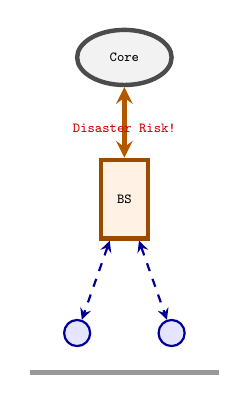
\begin{tikzpicture}[
            bs/.style={rectangle, fill=orange!10, draw=orange!60!black, ultra thick, minimum width=0.6cm, minimum height=1cm, align=center, font=\tiny\ttfamily},
            cloud/.style={draw, ellipse, fill=gray!10, draw=gray!60!black, ultra thick, minimum width=1.2cm, minimum height=0.7cm, font=\tiny\ttfamily},
            user/.style={circle, fill=blue!10, draw=blue!60!black, thick, minimum size=0.3cm},
            link/.style={<->, thick, >=stealth, gray!70},
            fiber/.style={link, ultra thick, orange!70!black},
            wireless/.style={link, dashed, blue!60!black}
        ]
            \node[cloud] (core) at (0,4) {Core};
            \node[bs] (bs) at (0,2.2) {BS};
            \node[user] (u1) at (-0.6,0.5) {};
            \node[user] (u2) at (0.6,0.5) {};

            \draw[fiber] (core) -- (bs);
            \draw[wireless] (bs) -- (u1);
            \draw[wireless] (bs) -- (u2);

            \draw[ultra thick, gray!80] (-1.2,0) -- (1.2,0);
            \node[red!80!black, font=\tiny\ttfamily] at (0,3.1) {Disaster Risk!};
        \end{tikzpicture}
        }
      \end{center}
    \end{column}
  \end{columns}
\end{frame}

\begin{frame}[c]{Ground Network}
  \begin{columns}[c]
    \begin{column}{0.6\textwidth}
      Ground networks consist of various networks. These networks realize wide-range and low-latency communication for users through base stations and access points.
      
      \vspace{0.5em}
      This network is the foundation of \texttt{SAGIN} and is characterized by its ability to provide abundant computational resources and high communication capacity.
      
      \vspace{0.5em}
      However, several limitations also exist. Coverage is limited to a few percent of the Earth due to geographical and economic issues. Furthermore, the risk from disasters is significant.
    \end{column}

    \begin{column}{0.35\textwidth}
      \begin{center}
        % 幅を倍に縮小
        \resizebox{0.7\linewidth}{!}{
        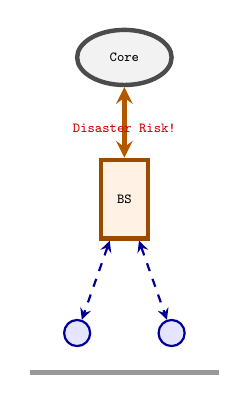
\begin{tikzpicture}[
            bs/.style={rectangle, fill=orange!10, draw=orange!60!black, ultra thick, minimum width=0.6cm, minimum height=1cm, align=center, font=\tiny\ttfamily},
            cloud/.style={draw, ellipse, fill=gray!10, draw=gray!60!black, ultra thick, minimum width=1.2cm, minimum height=0.7cm, font=\tiny\ttfamily},
            user/.style={circle, fill=blue!10, draw=blue!60!black, thick, minimum size=0.3cm},
            link/.style={<->, thick, >=stealth, gray!70},
            fiber/.style={link, ultra thick, orange!70!black},
            wireless/.style={link, dashed, blue!60!black}
        ]
            \node[cloud] (core) at (0,4) {Core};
            \node[bs] (bs) at (0,2.2) {BS};
            \node[user] (u1) at (-0.6,0.5) {};
            \node[user] (u2) at (0.6,0.5) {};

            \draw[fiber] (core) -- (bs);
            \draw[wireless] (bs) -- (u1);
            \draw[wireless] (bs) -- (u2);

            \draw[ultra thick, gray!80] (-1.2,0) -- (1.2,0);
            \node[red!80!black, font=\tiny\ttfamily] at (0,3.1) {Disaster Risk!};
        \end{tikzpicture}
        }
      \end{center}
    \end{column}
  \end{columns}
\end{frame}

\section{課題/Issues}

\begin{frame}{SAGINの課題/SAGIN's issues}
  \texttt{SAGIN}には様々な課題が存在する．主に以下のような問題である．
  \begin{itemize}
    \item トポロジー課題
    \item 資源管理
    \item セキュリティ
  \end{itemize}
  There are various challenges in \texttt{SAGIN}. The following are the main issues:
  \begin{itemize}
    \item Node and Topology Issues
    \item Resource Management
    \item Security
  \end{itemize}
\end{frame}

\subsection{トポロジー課題 / Topology}

\begin{frame}[c]{トポロジー課題}
  \begin{columns}[c]
    \begin{column}{0.6\textwidth}
      \texttt{SAGIN} における非地上の移動体機器は地上の基地局と比べても遥かに高い移動性能を持ってる．高速移動中にはネットワークトポロジが頻繁に変化する．

      \vspace{0.5em}
      それは，移動体のみの通信状態を考慮するだけでは通信を継続的に行うということは難しい．

      \vspace{0.5em}
      付近の建物の情報や天候状態，移動先の基地局の位置情報等を考えたうえでトポロジーを再編する必要がある．これらをできる限り短い時間で行わなければならない．
    \end{column}

    \begin{column}{0.35\textwidth}
      \begin{center}
        \resizebox{\linewidth}{!}{
        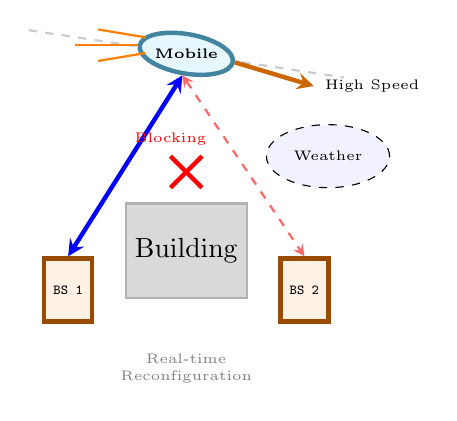
\begin{tikzpicture}[
            bs/.style={rectangle, fill=orange!10, draw=orange!60!black, ultra thick, minimum width=0.6cm, minimum height=0.8cm, font=\tiny\ttfamily},
            % 機体：少し傾けてスピード感を出す
            uav/.style={ellipse, fill=cyan!10, draw=cyan!60!black, ultra thick, minimum width=1.2cm, minimum height=0.5cm, rotate=-10},
            obs/.style={rectangle, fill=gray!30, draw=gray!60, thick, minimum width=0.5cm, minimum height=1.2cm},
            weather/.style={ellipse, draw, fill=blue!5, minimum width=1.2cm, minimum height=0.8cm, font=\tiny, dashed},
            link/.style={<->, thick, >=stealth, gray!70},
            active/.style={link, blue, ultra thick},
            future/.style={link, dashed, red!60},
            motion/.style={->, ultra thick, orange!80!black, >=stealth}
        ]
            % --- 飛行軌道（軌跡） ---
            \draw[dashed, gray!40, thick] (-2,3.8) -- (2,3.2);

            % --- ノード配置 ---
            \node[uav] (m) at (0,3.5) {};
            \node[font=\tiny\bfseries] at (0,3.5) {Mobile};

            % スピードライン（残像）
            \draw[orange, thick] (m.west) ++(0.1,0.1) -- ++(-0.6,0.1);
            \draw[orange, thick] (m.west) ++(0,0) -- ++(-0.8,0);
            \draw[orange, thick] (m.west) ++(0.1,-0.1) -- ++(-0.6,-0.1);

            \node[bs] (bs1) at (-1.5,0.5) {BS 1};
            \node[bs] (bs2) at (1.5,0.5) {BS 2};
            \node[obs] (bldg) at (0,) {Building};
            \node[weather] (rain) at (1.8,2.2) {Weather};

            % --- 動きのベクトル ---
            \draw[motion] (m.east) -- ++(1, -0.3) node[right, black, font=\tiny] {High Speed};

            % --- リンク ---
            \draw[active] (m.south) -- (bs1.north);
            \draw[future] (m.south) -- (bs2.north);

            % --- 遮蔽 ---
            \draw[red, ultra thick] (0.2,1.8) -- (-0.2,2.2) node[above, font=\tiny] {Blocking};
            \draw[red, ultra thick] (-0.2,1.8) -- (0.2,2.2);

            \node[font=\tiny, gray, align=center] at (0,-0.5) {Real-time \\ Reconfiguration};
        \end{tikzpicture}
        }
      \end{center}
    \end{column}
  \end{columns}
\end{frame}

\begin{frame}[c]{Topology Challenges}
  \begin{columns}[c]
    \begin{column}{0.6\textwidth}
      Non-terrestrial mobile equipment in \texttt{SAGIN} has significantly higher mobility compared to ground base stations. During high-speed movement, the network topology changes frequently.

      \vspace{0.5em}
      It is difficult to maintain continuous communication by considering only the status of the mobile devices themselves.

      \vspace{0.5em}
      The topology must be reconfigured by taking into account factors such as nearby buildings, weather conditions, and the location of destination base stations. These tasks must be performed in as short a time as possible.
    \end{column}

    \begin{column}{0.35\textwidth}
      \begin{center}
        \resizebox{\linewidth}{!}{
        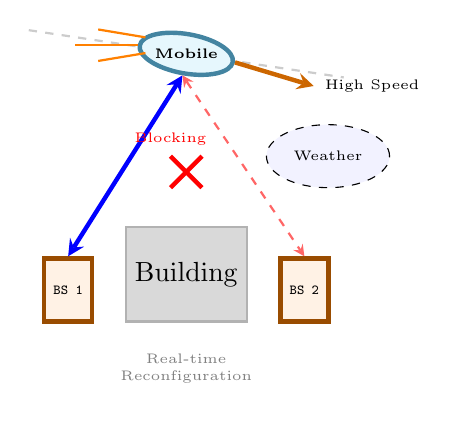
\begin{tikzpicture}[
            bs/.style={rectangle, fill=orange!10, draw=orange!60!black, ultra thick, minimum width=0.6cm, minimum height=0.8cm, font=\tiny\ttfamily},
            uav/.style={ellipse, fill=cyan!10, draw=cyan!60!black, ultra thick, minimum width=1.2cm, minimum height=0.5cm, rotate=-10},
            obs/.style={rectangle, fill=gray!30, draw=gray!60, thick, minimum width=0.5cm, minimum height=1.2cm},
            weather/.style={ellipse, draw, fill=blue!5, minimum width=1.2cm, minimum height=0.8cm, font=\tiny, dashed},
            link/.style={<->, thick, >=stealth, gray!70},
            active/.style={link, blue, ultra thick},
            future/.style={link, dashed, red!60},
            motion/.style={->, ultra thick, orange!80!black, >=stealth}
        ]
            % Trajectory
            \draw[dashed, gray!40, thick] (-2,3.8) -- (2,3.2);

            % Mobile Node
            \node[uav] (m) at (0,3.5) {};
            \node[font=\tiny\bfseries] at (0,3.5) {Mobile};

            % Speed Lines
            \draw[orange, thick] (m.west) ++(0.1,0.1) -- ++(-0.6,0.1);
            \draw[orange, thick] (m.west) ++(0,0) -- ++(-0.8,0);
            \draw[orange, thick] (m.west) ++(0.1,-0.1) -- ++(-0.6,-0.1);

            \node[bs] (bs1) at (-1.5,0.5) {BS 1};
            \node[bs] (bs2) at (1.5,0.5) {BS 2};
            \node[obs] (bldg) at (0,0.7) {Building};
            \node[weather] (rain) at (1.8,2.2) {Weather};

            % Motion Vector
            \draw[motion] (m.east) -- ++(1, -0.3) node[right, black, font=\tiny] {High Speed};

            % Links
            \draw[active] (m.south) -- (bs1.north);
            \draw[future] (m.south) -- (bs2.north);

            % Blocking
            \draw[red, ultra thick] (0.2,1.8) -- (-0.2,2.2) node[above, font=\tiny] {Blocking};
            \draw[red, ultra thick] (-0.2,1.8) -- (0.2,2.2);

            \node[font=\tiny, gray, align=center] at (0,-0.5) {Real-time \\ Reconfiguration};
        \end{tikzpicture}
        }
      \end{center}
    \end{column}
  \end{columns}
\end{frame}

\subsection{資源管理 / Resource Management}

\begin{frame}[c]{資源管理 / Resource Management}
  \begin{columns}[t]
    % --- 左側：日本語 ---
    \begin{column}{0.48\textwidth}
      \texttt{SAGIN} では，通信資源と計算資源を同時に管理する必要がある．衛星や \texttt{UAV} は，電力や計算能力が限られている．ノードが移動するため，通信経路が動的に変化する．

      \vspace{1em}
      主な最適化対象
      \begin{itemize}
        \item タスクオフロード
        \item 電力制御
        \item 帯域割当
        \item 通信経路選択
      \end{itemize}
    \end{column}

    % 中央に余白を確保
    \hfill
    \vrule
    \hfill

    % --- 右側：英語 ---
    \begin{column}{0.48\textwidth}
      In \texttt{SAGIN}, it is necessary to manage communication and computational resources simultaneously. Satellites and \texttt{UAV}s have limited power and computing capabilities.

      \vspace{1em}
      Optimization Targets
      \begin{itemize}
        \item Task Offloading
        \item Power Control
        \item Bandwidth Allocation
        \item Routing Selection
      \end{itemize}
    \end{column}
  \end{columns}
\end{frame}

\subsection{セキュリティ/Security}

\begin{frame}[c]{セキュリティ}
  \begin{columns}[c]
    \begin{column}{0.6\textwidth}
      \texttt{SAGIN} は開放的な通信環境や，動的なトポロジーなどからセキュリティは深刻なものである．

      \vspace{0.5em}
      様々な通信機器と通信を行うことから攻撃されるリスクや問題が波及することも考えられる．

      \vspace{0.5em}
      以下のセキュリティを備えている必要がある．
      \begin{itemize}
        \item 物理層セキュリティ
        \item 認証技術
        \item データの機密性とプライバシー
      \end{itemize}
    \end{column}

    \begin{column}{0.35\textwidth}
      \begin{center}
        \resizebox{\linewidth}{!}{
        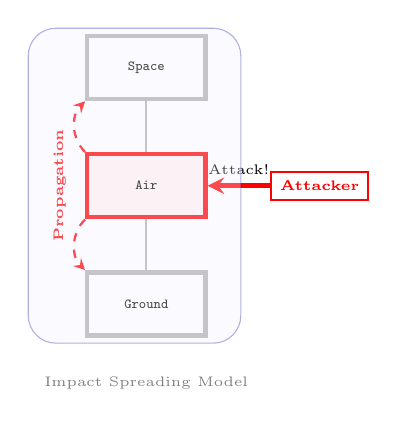
\begin{tikzpicture}[
            node/.style={rectangle, draw=gray!60, fill=white, ultra thick, minimum width=1.5cm, minimum height=0.8cm, font=\tiny\ttfamily},
            attack/.style={draw=red, ultra thick, ->, >=stealth},
            % 波及（プロパゲーション）用の赤い点線矢印
            prop/.style={draw=red, thick, dashed, ->, >=stealth},
            shield/.style={draw=blue!60!black, fill=blue!5, opacity=0.3, rounded corners=10pt},
            link/.style={thick, gray!60}
        ]
            % --- ノード配置 ---
            \node[node] (sat) at (0,3) {Space};
            \node[node, draw=red, fill=red!5] (uav) at (0,1.5) {Air}; % 攻撃を受けた中心
            \node[node] (gnd) at (0,0) {Ground};

            % --- 基本リンク ---
            \draw[link] (sat) -- (uav);
            \draw[link] (uav) -- (gnd);

            % --- 攻撃者 ---
            \node[red, font=\tiny\bfseries, draw=red, thick] (attacker) at (2.2,1.5) {Attacker};
            \draw[attack] (attacker.west) -- (uav.east) node[midway, above, font=\tiny, black] {Attack!};

            % --- 問題の波及 (Propagation) ---
            % AirからSpaceへ
            \draw[prop] (uav.north west) to[bend left=45] (sat.south west);
            % AirからGroundへ
            \draw[prop] (uav.south west) to[bend right=45] (gnd.north west);

            \node[red, font=\tiny\bfseries, rotate=90] at (-1.1,1.5) {Propagation};

            % --- 防護層 ---
            \draw[shield] (-1.5,-0.5) rectangle (1.2,3.5);

            \node[font=\tiny, gray, align=center] at (0,-1) {Impact Spreading Model};
        \end{tikzpicture}
        }
      \end{center}
    \end{column}
  \end{columns}
\end{frame}

\begin{frame}[c]{Security}
  \begin{columns}[c]
    \begin{column}{0.6\textwidth}
      Security is a critical issue for \texttt{SAGIN} due to its open communication environment and dynamic topology.

      \vspace{0.5em}
      Since it communicates with various devices, there is a risk of attacks and the spreading of issues throughout the network.

      \vspace{0.5em}
      It is necessary to implement the following security measures:
      \begin{itemize}
        \item Physical Layer Security
        \item Authentication Technology
        \item Data Confidentiality and Privacy
      \end{itemize}
    \end{column}

    \begin{column}{0.35\textwidth}
      \begin{center}
        \resizebox{\linewidth}{!}{
        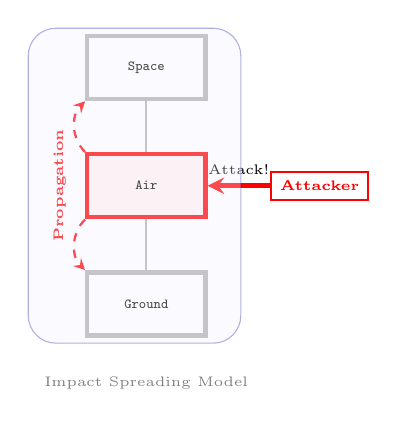
\begin{tikzpicture}[
            node/.style={rectangle, draw=gray!60, fill=white, ultra thick, minimum width=1.5cm, minimum height=0.8cm, font=\tiny\ttfamily},
            attack/.style={draw=red, ultra thick, ->, >=stealth},
            prop/.style={draw=red, thick, dashed, ->, >=stealth},
            shield/.style={draw=blue!60!black, fill=blue!5, opacity=0.3, rounded corners=10pt},
            link/.style={thick, gray!60}
        ]
            % --- Nodes ---
            \node[node] (sat) at (0,3) {Space};
            \node[node, draw=red, fill=red!5] (uav) at (0,1.5) {Air};
            \node[node] (gnd) at (0,0) {Ground};

            % --- Links ---
            \draw[link] (sat) -- (uav);
            \draw[link] (uav) -- (gnd);

            % --- Attacker ---
            \node[red, font=\tiny\bfseries, draw=red, thick] (attacker) at (2.2,1.5) {Attacker};
            \draw[attack] (attacker.west) -- (uav.east) node[midway, above, font=\tiny, black] {Attack!};

            % --- Propagation of Impact ---
            \draw[prop] (uav.north west) to[bend left=45] (sat.south west);
            \draw[prop] (uav.south west) to[bend right=45] (gnd.north west);

            \node[red, font=\tiny\bfseries, rotate=90] at (-1.1,1.5) {Propagation};

            % --- Shield ---
            \draw[shield] (-1.5,-0.5) rectangle (1.2,3.5);

            \node[font=\tiny, gray, align=center] at (0,-1) {Impact Spreading Model};
        \end{tikzpicture}
        }
      \end{center}
    \end{column}
  \end{columns}
\end{frame}

\begin{frame}[c]{物理層セキュリティ}
  \begin{columns}[c]
    \begin{column}{0.55\textwidth}
      宇宙・航空ネットワークでは，地上のような物理的な保護が困難なため，盗聴やジャミングに脆弱である．

      \begin{itemize}
        \item ジャミング攻撃 \\
          強力な干渉信号により正規リンクを遮断する．リソース制限により回避が困難．
        \item 物理層セキュリティ技術 \\
          複雑な暗号に頼らず，物理的特性で秘匿性を保証する．例：人工ノイズの付加．
      \end{itemize}
    \end{column}

    \begin{column}{0.42\textwidth}
      \begin{center}
        % カラム幅の0.7倍を維持
        \resizebox{\linewidth}{!}{
        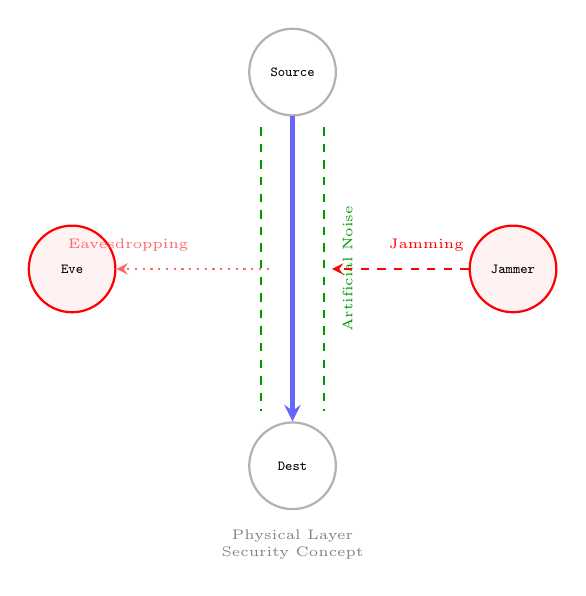
\begin{tikzpicture}[
            node/.style={circle, draw=gray!60, fill=white, thick, minimum size=1.1cm, font=\tiny\ttfamily},
            bad/.style={circle, draw=red, fill=red!5, thick, minimum size=1.1cm, font=\tiny\ttfamily},
            link/.style={->, >=stealth, ultra thick, blue!60},
            % ジャミング矢印を細く修正 (ultra thick -> thick)
            jam/.style={->, >=stealth, thick, red, dashed},
            noise/.style={draw=green!60!black, thick, dashed}
        ]
            % --- ノード ---
            \node[node] (alice) at (0,4.5) {Source};
            \node[node] (bob) at (0,-0.5) {Dest};
            \node[bad] (jammer) at (2.8,2) {Jammer};
            \node[bad] (eve) at (-2.8,2) {Eve};

            % --- 正規通信 ---
            \draw[link] (alice) -- (bob);
            
            % 人工ノイズ（緑色文字が矢印の下でも読めるように）
            \draw[noise, green!60!black] (-0.4,3.8) -- (-0.4,0.2);
            \draw[noise, green!60!black] (0.4,3.8) -- (0.4,0.2);
            \node[green!60!black, font=\tiny, rotate=90] at (0.7,2) {Artificial Noise};

            % --- 攻撃 ---
            \draw[jam] (jammer) -- (0.5,2); % スタイル jam が細くなっている
            % ジャミングラベルの位置を左に修正 (at (1.5) -> at (1.1))
            \node[red, font=\tiny, anchor=west] at (1.1,2.3) {Jamming};
            
            % 盗聴
            \draw[->, >=stealth, thick, red!60, dotted] (-0.3,2) -- (eve);
            \node[red!60, font=\tiny, anchor=east] at (-1.2,2.3) {Eavesdropping};

            % キャプション
            \node[font=\tiny, gray, align=center] at (0,-1.5) {Physical Layer \\ Security Concept};
        \end{tikzpicture}
        }
      \end{center}
    \end{column}
  \end{columns}
\end{frame}

\begin{frame}[c]{Physical Layer Security}
  \begin{columns}[c]
    \begin{column}{0.55\textwidth}
      Space and aerial networks are vulnerable to eavesdropping and jamming attacks because physical protection is difficult.

      \begin{itemize}
        \item Jamming Attack \\
          Malicious nodes block legitimate links with strong interference. It is hard to avoid due to resource constraints.
        \item Security Technology \\
          Ensures confidentiality using physical characteristics instead of complex crypto. Example: Artificial Noise (AN).
      \end{itemize}
    \end{column}

    \begin{column}{0.42\textwidth}
      \begin{center}
        \resizebox{\linewidth}{!}{
        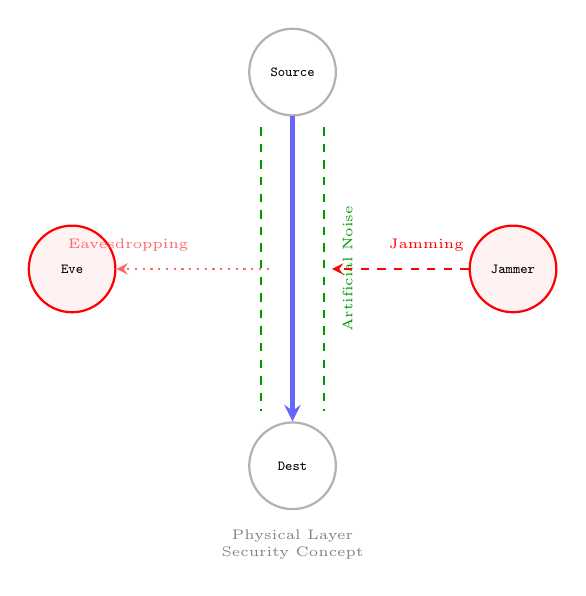
\begin{tikzpicture}[
            node/.style={circle, draw=gray!60, fill=white, thick, minimum size=1.1cm, font=\tiny\ttfamily},
            bad/.style={circle, draw=red, fill=red!5, thick, minimum size=1.1cm, font=\tiny\ttfamily},
            link/.style={->, >=stealth, ultra thick, blue!60},
            % Thin jamming arrow
            jam/.style={->, >=stealth, thick, red, dashed},
            noise/.style={draw=green!60!black, thick, dashed}
        ]
            % --- Nodes ---
            \node[node] (alice) at (0,4.5) {Source};
            \node[node] (bob) at (0,-0.5) {Dest};
            \node[bad] (jammer) at (2.8,2) {Jammer};
            \node[bad] (eve) at (-2.8,2) {Eve};

            % --- Legitimate Link ---
            \draw[link] (alice) -- (bob);

            % Artificial Noise (green text is readable beneath the thin arrow)
            \draw[noise, green!60!black] (-0.4,3.8) -- (-0.4,0.2);
            \draw[noise, green!60!black] (0.4,3.8) -- (0.4,0.2);
            \node[green!60!black, font=\tiny, rotate=90] at (0.7,2) {Artificial Noise};

            % --- Attacks ---
            \draw[jam] (jammer) -- (0.5,2);
            % Shifted Jamming label left (at (1.5) -> at (1.1))
            \node[red, font=\tiny, anchor=west] at (1.1,2.3) {Jamming};

            \draw[->, >=stealth, thick, red!60, dotted] (-0.3,2) -- (eve);
            \node[red!60, font=\tiny, anchor=east] at (-1.2,2.3) {Eavesdropping};

            \node[font=\tiny, gray, align=center] at (0,-1.5) {Physical Layer \\ Security Concept};
        \end{tikzpicture}
        }
      \end{center}
    \end{column}
  \end{columns}
\end{frame}

\begin{frame}[c]{認証技術}
  \begin{columns}[c]
    \begin{column}{0.6\textwidth}
      \texttt{SAGIN} では，通信が航空，宇宙などの異なるレイヤや基地局，プラットフォーム間を頻繁に移動するため高速かつ安全な認証メカニズムが必要である．
      
      \begin{itemize}
        \item クロスレイヤ認証 \\
          異なる通信レイヤ間を移動する際に再認証の遅延を最小限に抑える必要がある．従来の方法では宇宙ネットワークのような長い遅延下では効率が低下する．
        \item 分散型認証 \\
          中央サーバに依存しない形での認証プロトコルが必要である．そのためにブロックチェーンや分散型台帳技術を利用した方法などによって信頼性向上などが考えられている．
      \end{itemize}
    \end{column}

    \begin{column}{0.35\textwidth}
      \begin{center}
        % 再度 0.7倍に縮小してバランスを調整
        \resizebox{0.7\linewidth}{!}{
        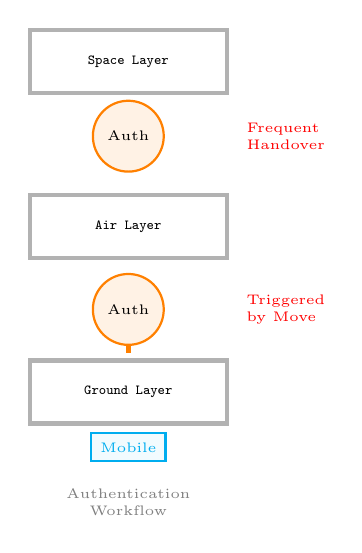
\begin{tikzpicture}[
            node/.style={rectangle, draw=gray!60, fill=white, ultra thick, minimum width=2.5cm, minimum height=0.8cm, font=\tiny\ttfamily},
            auth/.style={circle, draw=orange, fill=orange!10, thick, minimum size=0.9cm, font=\tiny, align=center},
            link/.style={->, >=stealth, orange, ultra thick, dashed}
        ]
            % --- 各レイヤ ---
            \node[node] (space) at (0,4.2) {Space Layer};
            \node[node] (air) at (0,2.1) {Air Layer};
            \node[node] (gnd) at (0,0) {Ground Layer};

            % --- 移動と認証のトリガー ---
            \draw[link] (0,0.5) -- (0,1.4);
            \node[auth] (check1) at (0,1.05) {Auth};

            \draw[link] (0,2.8) -- (0,3.7);
            \node[auth] (check2) at (0,3.25) {Auth};

            % 移動体の簡略表示
            \node[draw, cyan, fill=cyan!5, thick, minimum width=0.8cm] at (0,-0.7) {\tiny Mobile};

            % 右側のラベルをコンパクトに
            \node[red, font=\tiny, align=left] at (2.0,1.05) {Triggered\\by Move};
            \node[red, font=\tiny, align=left] at (2.0,3.25) {Frequent\\Handover};

            \node[font=\tiny, gray, align=center] at (0,-1.4) {Authentication \\ Workflow};
        \end{tikzpicture}
        }
      \end{center}
    \end{column}
  \end{columns}
\end{frame}

\begin{frame}[c]{Authentication Technology}
  \begin{columns}[c]
    \begin{column}{0.6\textwidth}
      In \texttt{SAGIN}, a fast and secure authentication mechanism is required as communication frequently moves between different layers, base stations, and platforms such as aerial and space.

      \begin{itemize}
        \item Cross-layer Authentication \\
          It is necessary to minimize re-authentication delay when moving between different communication layers. Conventional methods decrease in efficiency under long delays like space networks.
        \item Distributed Authentication \\
          Authentication protocols that do not rely on a central server are required. To achieve this, methods using blockchain or distributed ledger technology are being considered to improve reliability.
      \end{itemize}
    \end{column}

    \begin{column}{0.35\textwidth}
      \begin{center}
        \resizebox{0.7\linewidth}{!}{
        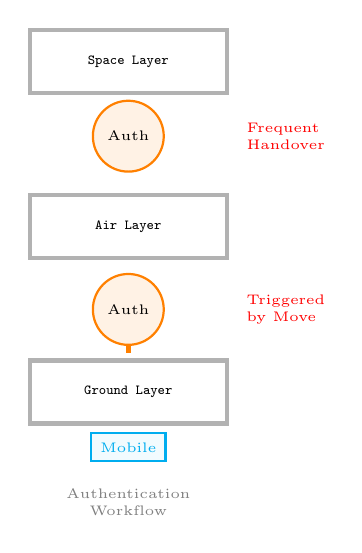
\begin{tikzpicture}[
            node/.style={rectangle, draw=gray!60, fill=white, ultra thick, minimum width=2.5cm, minimum height=0.8cm, font=\tiny\ttfamily},
            auth/.style={circle, draw=orange, fill=orange!10, thick, minimum size=0.9cm, font=\tiny, align=center},
            link/.style={->, >=stealth, orange, ultra thick, dashed}
        ]
            % --- Layers ---
            \node[node] (space) at (0,4.2) {Space Layer};
            \node[node] (air) at (0,2.1) {Air Layer};
            \node[node] (gnd) at (0,0) {Ground Layer};

            % --- Mobility & Auth Triggers ---
            \draw[link] (0,0.5) -- (0,1.4);
            \node[auth] (check1) at (0,1.05) {Auth};

            \draw[link] (0,2.8) -- (0,3.7);
            \node[auth] (check2) at (0,3.25) {Auth};

            \node[draw, cyan, fill=cyan!5, thick, minimum width=0.8cm] at (0,-0.7) {\tiny Mobile};

            \node[red, font=\tiny, align=left] at (2.0,1.05) {Triggered\\by Move};
            \node[red, font=\tiny, align=left] at (2.0,3.25) {Frequent\\Handover};

            \node[font=\tiny, gray, align=center] at (0,-1.4) {Authentication \\ Workflow};
        \end{tikzpicture}
        }
      \end{center}
    \end{column}
  \end{columns}
\end{frame}

\begin{frame}[c]{データの機密性とプライバシー}
  \texttt{SAGIN} を流れるデータには，軍事情報や個人の位置情報などの機密情報が含まれるため，高度な保護が必要である．

  \vspace{1.5em}

  \begin{itemize}
    \item プライバシー保護コンピューティング \\
      衛星や航空機をデータセンターとして利用する際，データを隠したまま処理する秘密計算や準同型暗号の適用が研究されている．
      
    \vspace{1em}
    
    \item 位置プライバシー \\
      特に \texttt{UAV} や \texttt{LEO} 衛星を介した通信では，ユーザーの地理的位置が特定されないよう，匿名化や差分プライバシーの導入が求められる．
  \end{itemize}
\end{frame}

\begin{frame}[c]{Data Confidentiality and Privacy}
  Data transmitted over \texttt{SAGIN} includes sensitive information such as military data and individual location info, requiring high-level protection.

  \vspace{1.5em}

  \begin{itemize}
    \item Privacy-Preserving Computing \\
      When using satellites or aircraft as data centers, research is being conducted on secret computing and homomorphic encryption to process data while keeping it hidden.

    \vspace{1em}

    \item Location Privacy \\
      Especially in communications via \texttt{UAV} or \texttt{LEO} satellites, anonymization and differential privacy are required to prevent the user's geographic location from being identified.
  \end{itemize}
\end{frame}

\begin{frame}[c]{参考文献 / References}
  \begin{thebibliography}{9}
    % \bibitem{ラベル} の形式で定義します
    \bibitem{chen2023space}
      N. Chen, B. Yang, Y. Zhang, and X. Guan,
      "Space-Air-Ground Integrated Network (SAGIN): A Survey,"
      arXiv preprint arXiv:2307.14697, 2023. \\
      \texttt{https://arxiv.org/abs/2307.14697}
  \end{thebibliography}
\end{frame}

\end{document}
